\documentclass{article}
\usepackage{graphicx} % Required for inserting images
\usepackage[spanish]{babel}
\usepackage{amssymb}
\usepackage{amsmath}
\usepackage{algorithm}
\usepackage{algpseudocode}
\usepackage{booktabs}
\usepackage{tabularx}
\usepackage{float}
\usepackage{booktabs}
\usepackage{xcolor}
\usepackage{makecell}
\usepackage{url}
\floatname{algorithm}{Algoritmo}


\title{Taller de Multiple Importance Sampling}
\author{Santiago Olmedo}
\date{Febrero 2024}

\begin{document}
\AddToHook{cmd/section/before}{\clearpage}

\maketitle

\section{Introducción}

En computación gráfica, los problemas de renderizado de imágenes se definen a través de la resolución de problemas de integración. Por ejemplo, la Ecuación de Rendering, ecuación~\ref{eq:rendering}, que se describe como una integral de Fredholm de segunda especie, de carácter recursivo. Esta ecuación presenta la particularidad de incluir la función incógnita en ambos lados de la igualdad, lo que conlleva a su resolución aproximada mediante procesos iterativos.

\begin{equation} \label{eq:rendering}
I(x,x') = g(x,x') \left[ e(x,x') + \int_{S} \rho(x,x',x'')I(x',x'') \, dx'' \right]
\end{equation}

donde:
\begin{itemize}
    \item \( I(x,x') \) es la intensidad de la luz que pasa del punto \( x' \) al punto \( x \).
    \item \( g(x,x') \) es un término geométrico.
    \item \( e(x,x') \) se refiere a la intensidad de luz emitida desde \( x' \) hacia \( x \).
    \item \( \rho(x,x',x'') \) se relaciona con la intensidad de luz dispersada desde \( x'' \) por una superficie en \( x' \).
\end{itemize}


Comúnmente, estás integrales son "difíciles", es decir, las funciones a integrar son discontinuas, multidimensionales o singulares y en general no poseen soluciones analíticas.
Es por ello que se recurre a métodos de resolución numéricos que permiten aproximar el valor de la integral con baja varianza.
Por la naturaleza de los problemas de renderizado, donde por ejemplo, se requiere calcular la luz de cada píxel de una imagen en tiempo real, es necesario que los métodos de resolución sean eficientes en tiempo de ejecución y errores de estimación.
Los métodos comunes, como la integración trapezoidal o cuadratura de Gauss son efectivos para la resolución de problemas de baja dimensión pero no son escalables a los problemas que aparecen en computación gráfica.
La integración por Monte Carlo es particularmente atractivo porque su convergencia es independiente de la dimensionalidad del problema.

Otro atractivo del método de Monte Carlo es su facilidad de implementación. A priori, dado

$$ \int f(x) \,d(x)$$

solo se necesita la capacidad de evaluar $f(x)$ en un punto dado para poder estimar el valor de la integral.

Debido a los problemas de integración que aparecen en computación gráfica, es necesario recurrir a métodos de Monte Carlo que permitan reducir la varianza de la estimación.

En este trabajo se presenta la técnica de Multiple Importance Sampling (MIS) que permite combinar múltiples distribuciones de muestreo para reducir la varianza de la estimación.

El informe está organizado de la siguiente manera:
\begin{itemize}
\item En la sección 2 se presenta el método de Monte Carlo.
\item En la sección 3 se presenta la técnica de Multiple Importance Sampling y un estudio del estado del arte.
\item En la sección 4 se presenta la implementación de MIS en un conjunto de pruebas que permiten analizar el comportamiento de MIS en distintos escenarios.
Esta comparación se basa en los errores de la estimación, el número de muestras requeridas y la variabilidad de las estimaciones (estimación de la varianza).
\item En la sección 5 se presentan las conclusiones del informe.
\end{itemize}

\section{Monte Carlo}

En general, los métodos numéricos que se fundamentan en la evaluación de \( n \) puntos dentro de un espacio de dimensión \( m \) para obtener una solución aproximada presentan un error que disminuye en el mejor de los casos en proporción a \( n^{-1/m} \).
Esta característica los hace extremadamente ineficientes en situaciones donde \( m \) es grande.

Por otro lado, los métodos de Monte Carlo generan estimaciones cuyo error absoluto es del orden de \( n^{-1/2} \), independientemente de la dimensión \( m \). Esta cualidad representa la ventaja principal del método y, en muchos casos, hace que sea la única opción viable.

Supongamos que deseo calcular un cierto valor $\phi$, y conozco una variable aleatoria $X$ con distribución $F_X$ tal que $\phi = \mathbb{E}(X)$. El método de Monte Carlo en su versión más simple consiste en:

\begin{algorithm}
\caption{Esquema básico de un Método Monte Carlo}
\begin{algorithmic}[1]

\State \textbf{sortear} valores para un conjunto $X^{(1)}, X^{(2)}, \dots, X^{(n)}$, de variables aleatorias i.i.d. (independientes e idénticamente distribuidas) a $X$.

\State Calcular $S_n = X^{(1)} + \dots + X^{(n)}$, la suma de los $n$ valores sorteados.

\State Calcular $\hat{X} = \frac{S_n}{n}$.

\State Calcular $\hat{V} = \left(\sum_{i=1}^{n} (X^{(i)})^2\right) / (n(n - 1)) - \hat{X}^2 / (n - 1)$.

\end{algorithmic}
\end{algorithm}

Se dice que $\hat{X}$ es un estimador de $\phi$ y $\hat{V}$ es un estimador de la varianza de $\hat{X}$.

Ahora, supongamos que se quiere evaluar el valor de la integral $I = \int_{a}^{b} f(x) \,dx$. Dado un conjunto de $n$ variables aleatorias $X_1, X_2, \dots, X_n$ independientes e idénticamente distribuidas con distribución uniforme $p(x)$, se puede decir que el valor esperado del estimador
$$F = \frac{b-a}{n} \sum_{i=1}^{n} f(X_i)$$
es igual a $I$. Esto se puede ver de la siguiente manera:
$$E[F] = E\left[\frac{b-a}{n} \sum_{i=1}^{n} f(X_i)\right] = \frac{b-a}{n} \sum_{i=1}^{n} E[f(X_i)] = \frac{b-a}{n} \sum_{i=1}^{n} \int_{a}^{b} f(x) p(x) \,dx = \int_{a}^{b} f(x) \,dx.$$
Dado que $X_i$ es muestreado de $[a,b]$, $p(x) = \frac{1}{b-a}$ para $x \in [a,b]$. Entonces, sustituyendo $p(x)$ por $\frac{1}{b-a}$, y haciendo $\frac{b-a}{n} n = b-a$, se cancela con $\frac{1}{b-a}$, y se obtiene la última igualdad.

La restricción de usar distribuciones uniformes se puede sacar haciendo una generalización. Para una distribución arbitraria $p(x)$ que satisface que sea distinto de 0 para todo $x$ donde $f(x)$ es distinto de 0, se puede decir que el valor esperado del estimador
$$ F = \frac{1}{n} \sum_{i=1}^{n} \frac{f(X_i)}{p(X_i)}$$
se puede usar para estimar la integral I. De manera parecida, se puede ver que el valor esperado del estimador es igual a I:
$$E[F] = E\left[\frac{1}{n} \sum_{i=1}^{n} \frac{f(X_i)}{p(X_i)}\right] = \frac{1}{n} \sum_{i=1}^{n} \int_{a}^{b} \frac{f(x)}{p(x)} p(x) \,dx = \frac{1}{n} \sum_{i=1}^{n} \int_{a}^{b} f(x) \,dx = \int_{a}^{b} f(x) \,dx$$

Ahora, es importante mostrar el error de la estimación. Para esto, se puede usar el estimador del esquema básico de Monte Carlo para la varianza de $F$:

$$V[\frac{1}{n}\sum_{i=1}^{n} X_{(i)}] = \frac{1}{n^{2}} \sum_{i=1}^{n} V[X_{(i)}]$$

dado que las variables aleatorias $X_{i}$ son independientes. Teniendo en cuenta que $X_{i}$ tienen la misma distribución y por lo tanto la misma desviación estándar, se puede escribir la varianza del estimador $F$ como:

$$V[F] = \frac{1}{n^{2}} \sum_{i=1}^{n} V[X_{i}] = \frac{1}{n^{2}} \cdot n \cdot \sigma^{2} = \frac{\sigma^{2}}{n}.$$

Sin embargo, el error estándar del estimador, que proporciona una medida de la precisión de la estimación de $\phi$, se calcula como la raíz cuadrada de esta varianza, resultando en:

$$\text{Error estándar} = \sqrt{\frac{\sigma^{2}}{n}} = \frac{\sigma}{\sqrt{n}}.$$

Por lo tanto, el error de la estimación disminuye a una tasa de $n^{-1/2}$, reflejando la precisión de la estimación del valor esperado $\phi$ en términos de la desviación estándar $\sigma$.

\section{Multiple Importance Sampling}

En esta sección se va a presentar la técnica de Multiple Importance Sampling (MIS) y un estudio del estado del arte.

\subsection{Motivación}

Según vimos en la sección anterior, el método de Monte Carlo nos provee de un buen estimador para la integral de una función.
Ahora, cuando nos enfrentamos a problemas de computación gráfica donde la función a integrar puede ser compleja como la ecuación de rendering necesitamos más muestras para obtener una estimación precisa.
La cantidad de muestras trae consigo un costo computacional y por lo tanto se buscan técnicas que permitan mejorar la eficiencia de la estimación.

\paragraph{Importance Sampling}
Una de las técnicas que se pueden usar para mejorar la eficiencia de la estimación es Importance Sampling (IS).

Esta técnica consiste en, dado el estimador de Monte Carlo

$$ F = \frac{1}{n} \sum_{i=1}^{n} \frac{f(X_{i})}{p(X_{i})}$$

aprovechar que la varianza de $F$ se puede reducir si se elige una distribución de muestreo $p(x)$ que sea cercana a $f(x)$.

La clave para reducir la varianza del estimador con Importance Sampling recae en la elección de la distribución de muestreo $p(x)$.
Al seleccionar una $p(x)$ que sea cercana a $f(x)$, se logra que las muestras generadas $X_{i}$ se concentren en las regiones donde $f(x)$ es más grande lo que resulta en:

\begin{itemize}
    \item Al enfocarse más en las áreas donde $f(x)$ tiene valores más altos, cada muestra contribuye más información útil para la estimación.
          Esto hace que el estimador sea más eficiente con menos muestras.
    \item Las muestras no se desperdician en regiones donde $f(x)$ contribuye poco y nada al valor de la integral.
\end{itemize}

\paragraph{Multiple Importance Sampling}

En este caso, tenemos una integral que puede ser de de la forma
$$ \int f_{1}(x) f_{2}(x) f_{3}(x) ... f_{k}(x) \,d(x)$$

y $ p_{1}, p_{2}, p_{3}, ..., p_{k}$ parecidas a $f_{1}, f_{2}, f_{3}, ..., f_{k}$.
La idea es usar las distintas distribuciones de muestreo y combinarlas para encontrar una estimación de la integral con menor varianza y y con bajo costo computacional.

El problema también es que la inherencia de la computación gráfica hace que las funciones a integrar dependan de varios parámetros del modelo de la escena.
Esto hace que sea difícil encontrar una distribución de muestreo que sea buena para todos los parámetros.
Por lo tanto, se puede usar MIS para combinar varias distribuciones de muestreo y obtener una estimación con menor varianza para todo el espacio de parámetros.

En las próximas subsecciones se van a presentar las técnicas para combinar las distribuciones de muestreo.
Se asume que ya están definidas las distribuciones de muestreo y a partir de estas se construyen estimadores con baja varianza.

Veach, en su tesis de doctorado \cite{Veach1997} introduce el concepto de MIS y presenta técnicas para combinar las distribuciones y obtener un estimador con varianza baja y demostrablemente bueno.
En su tesis presenta el modelo multi-sample y distintas heurísticas para combinar las distribuciones de muestreo.
A su vez, presenta el modelo one-sample que consiste en elegir en cada ejecución una distribución de muestreo y usarla para estimar la integral.

\subsection{Modelo multi-sample}

Sea la siguiente integral que se quiere estimar:

$$ \int f(x) \,d\mu(x)$$

donde el dominio de integración es $\Omega$ y $\mu$ es dado. Tenemos $n$ distribuciones de muestreo $p_{1}, p_{2}, ..., p_{n}$, en el dominio $\Omega$.
Tenemos las siguientes operaciones:
\begin{itemize}
    \item dado $x \in \Omega$, podemos evaluar $f(x)$ y $p_{i}(x)$.
    \item la posibilidad de generar una muestra X con distribución $p_{i}$ para $i \in \{1, 2, ..., n\}$.
\end{itemize}

Notación:
\begin{itemize}
    \item $n_{i}$: número de muestras generadas con $p_{i}$. Este numéro es conocido a priori.
    \item $N = \sum_{i=1}^{n} n_{i}$: número total de muestras.
    \item Para $j \in \{1, 2, ..., N\}$, $X_{i,j}$ es la $j$-ésima muestra generada con $p_{i}$.
\end{itemize}

\subsection{Estimador multi-sample}

Objetivo: encontrar un estimador insesgado combinando las muestras generadas con las distintas distribuciones de muestreo.
Para esto, consideramos estimadores que le dan pesos diferentes a cada muestra.
El estimador multi-sample es de la forma:

$$F = \sum_{i=1}^{n} \frac{1}{n_{i}} \sum_{j=1}^{n_{i}} w_{i}(X_{i,j}) \frac{f(X_{i,j})}{p_{i}(X_{i,j})}$$

donde se tienen que cumplir las siguientes condiciones:

\begin{itemize}
    \item $\sum_{i=1}^{n} w_{i}(x) = 1$ si $f(x) \neq 0$
    \item $w_{i}(x) = 0$ si $p_{i}(x) = 0$
\end{itemize}

Esto implica que en cada punto donde f(x) es distinto de 0, al menos una de las distribuciones $p_{i}(x)$ es positiva.

\textbf{Lema 9.1} Sea $F$ el estimador multi-sample. Entonces, $F$ es insesgado, es decir:

$$E[F] = \int f(x) \,d\mu(x)$$

Podemos demostrar que:
\begin{align*}
E[F] &= E\left[\sum_{i=1}^n \frac{1}{n_i} \sum_{j=1}^{n_i} w_i(X_{i,j}) \frac{f(X_{i,j})}{p_i(X_{i,j})}\right] \\
&= \sum_{i=1}^n \frac{1}{n_i} E\left[\sum_{j=1}^{n_i} w_i(X_{i,j}) \frac{f(X_{i,j})}{p_i(X_{i,j})}\right] \\
&= \sum_{i=1}^n \frac{1}{n_i} \sum_{j=1}^{n_i} \int_{\Omega} w_i(x) \frac{f(x)}{p_i(x)} p_i(x) d\mu(x) \\
&= \int_{\Omega} \left(\sum_{i=1}^n w_i(x)\right) f(x) d\mu(x) \\
&= \int_{\Omega} f(x) d\mu(x),
\end{align*}
dado que por la primera condición mencionada, \( \sum_{i=1}^n w_i(x) = 1 \) siempre que \( f(x) \neq 0 \).

Por lo tanto, el estimador \( F \) es insesgado.

\subsection{\textit{Balance Heuristic}}

$$ \hat{w}_{i}(x) = \frac{n_{i} p_{i}(x)}{\sum_{k} n_{k} p_{k}(x)}$$

\textbf{Teorema 9.2} Dado $f$, $n_{i}$ y $p_{i}$ para $i \in \{1, 2, ..., n\}$. Sea F cualquier estimador insesgado de la forma del multi-sample estimator y $\hat{F}$ el estimador \textit{balance heuristic}. Entonces:

$$V[\hat{F}] - V[F] \leq ( \frac{1}{min_{i} n_{i}} - \frac{1}{\sum_{i} n_{i}} ) \mu^{2}$$

donde $\mu = E[F] = E[\hat{F}]$.

\subsection{Otras Heurísticas}

Dentro de los límites presentados en el Teorema 9.2, Veach presenta más heurísticas que son demostrablemente mejores que \textit{balance heuristic} en circunstancias particulares.
Estas heurísticas son insesgadas al igual que \textit{balance heuristic}.

Se considera la situación donde una de las distribuciones de muestreo es una muy buena aproximación a la función a integrar (ver figura \ref{fig:misother}).
En este caso, es deseable que la heurística le de un peso de 1 a esta distribución de muestreo y 0 a las demás.
La idea entonces es ir muestreando con las distintas distribuciones de muestreo y darle un peso de 1 en todo el dominio a la distribución de muestreo cercana a $f$ y 0 a las demás.
Sería como tomar muestras solo de la distribución de muestreo cercana a $f$ pero de igual manera tomando muestras de todas porque no se sabe de antemano cuál es la distribución de muestreo cercana a $f$.

\begin{figure}[H]
\centering
\includegraphics[width=0.6\textwidth]{Screenshot_mis.png}
\caption{Función f con las dos funciones de densidad $p_{1}$ y $p_{2}$}
\label{fig:misother}
\end{figure}

Para encontrar la heurística se toma como ejemplo la función donde $p_{1}$ es una coincidencia muy buena para $f$ y $p_{2}$ es una constante.
Se quiere encontrar una heurística donde los pesos sean:
$$w^{*}_{1}(x) \equiv 1$$
$$w^{*}_{2}(x) \equiv 0$$
ya que estos pesos nos darían una estimación $F^{*}$ con varianza 0.
Se puede apreciar un ejemplo de esto en la Figura \ref{fig:misother}.

\begin{figure}[H]
\centering
\includegraphics[width=0.6\textwidth]{Screenshot_mis2.png}
\caption{El dominio de integración se divide en dos regiones A y B.}
\label{fig:misother2}
\end{figure}

Ahora se presentan distintas heurísticas que tienen mejor rendimiento en las circunstancias mencionadas.
Como se muestra en la Figura \ref{fig:misother2}, el dominio de integración se divide en dos regiones A y B.

La observación que se puede hacer es que la mayoría de las muestras de $p_{1}$ caen en la región A donde $p_{1} > p_{2}$.
Se desea que en esta región las muestras de $p_{1}$ tengan un peso de 1 y las de $p_{2}$ un peso de 0.
\textit{balance heuristic} usaría el peso
$$ \hat{w}_{1}(x) = \frac{p_1}{p_1 + p_2} $$
que es mayor que 1/2 en la región A. Una manera de mejorar esto sería usando los pesos $w_{1}$ y $w_{2}$ que son 1 y 0 cada vez qie $\hat{w}_{1}$ es mayor que 1/2.

Veach propone dos combinaciones diferentes que aplican la idea de arriba. La primera es \textit{cutoff heuristic} y la segunda es \textit{power heuristic}.
Cada una pertenece a una familia de heurísticas controladas por un parámetro.
Por facilidad se reescriben los pesos de \textit{balance heuristic} como:
$$ \hat{w}_{i}(x) = \frac{q_{i}}{\sum_{k} q_{k}} $$

donde $q_{i} = n_{i} p_{i}$.

\paragraph{\textit{cutoff heuristic}} La heurística \textit{cutoff heuristic} es de la forma:
$$ w_{i}(x) = \begin{cases} 0 & \text{si } q_{i} < \alpha \cdot q_{max} \\ \frac{q_{i}}{\sum_{k} \{ q_{k} | q_{k} \geq \alpha \cdot q_{max} \}} & \text{en otro caso} \end{cases}$$

donde $q_{max} = max_{k} q_{k}$ y $\alpha$ es un parámetro que se elige de antemano $\in [0, 1]$.
El parámetro $\alpha$ define que tan grande tiene que ser $q_{i}$ para que la muestra tenga un peso distinto de 0.

\paragraph{\textit{power heuristic}} La heurística \textit{power heuristic} es de la forma:
$$ w_{i}(x) = \frac{(q_{i})^{\beta}}{\sum_{k} (q_{k})^{\beta}}$$

donde Veach recomienda $\beta = 2$.

Se puede ver que \textit{balance heuristic} se puede obtener cuando los parámetros $\alpha = 0$ o $\beta = 1$.
La otra heurística que surge de las anteriores 2 es la huerística \textit{maximum heuristic} cuando $\alpha = 1$ o $\beta = \infty$.

\paragraph{\textit{maximum heuristic}} La heurística \textit{maximum heuristic} es de la forma:
$$ w_{i}(x) = \begin{cases} 1 & \text{si } q_{i} = q_{max} \\ 0 & \text{en otro caso} \end{cases}$$

Lo que se hace es darle un peso de 1 a la distribución de muestreo que tiene el máximo $q_{i}$ y 0 a las demás.
Veach recomienda usar \textit{cutoff heuristic} y \textit{power heuristic} en lugar de \textit{maximum heuristic} ya que \textit{maximum heuristic} desecha muchas muestras.

\subsection{Modelo one-sample}

El modelo one-sample consiste en elegir en cada ejecución una distribución de muestreo de manera aleatoria y usarla para estimar la integral.
Dadas las distribuciones de muestreo $p_{1}, p_{2}, ..., p_{n}$, se elige una distribución de muestreo $p_{i}$ con probabilidades $c_{1}, c_{2}, ..., c_{n}$ (donde $\sum_{i} c_{i} = 1$).

El estimador one-sample es de la forma:
$$F = \frac{w_{I}(X_{I}) f(X_{I})}{c_{I} p_{I}(X_{I})}$$

donde $X_{I}$ es una muestra generada con $p_{I}$ y $I$ es una variable aleatoria con distribución $c_{1}, c_{2}, ..., c_{n}$.

\subsection{Enfoque de Sbert}

Sbert, en su artículo \cite{Sbert2016} presenta un enfoque diferente donde propone un cambio: en lugar de utilizar las mismas cantidad de muestras para todas las distribuciones de muestreo, se utilizan distintas cantidades de muestras para cada distribución de muestreo.
Esto, a grandes rasgos, se hace de la siguiente manera: las distribuciones con menor desviación estándar se muestrean con menos muestras y las distribuciones con mayor desviación estándar se muestrean con más muestras.

El enfoque de Sbert se basa en la idea de que las distribuciones de muestreo con menor desviación estándar contribuyen más a la estimación de la integral.
Sbert presenta los siguientes teoremas en su artículo:

\textbf{Teorema 1:} Dadas de números de muestras \(\{n_i\}\) y varianzas \(\{\sigma^2_i\}\), la disposición que minimiza (maximiza) la varianza \(V[F]\) es aquella que asocia las secuencias \(\{n_i\}\) y \(\{\sigma^2_i\}\) en el mismo orden (orden inverso), respectivamente.

\textbf{Teorema 2:} Si las varianzas \(\{\sigma^2_i\}\) son independientes del número de muestras, entonces la distribución \(\{n_i\}\) que minimiza la varianza \(V[F]\) es proporcional a las raíces cuadradas de las varianzas \(\sigma_i\).

\textbf{Teorema 3:} Si las varianzas \(\{\sigma^2_i\}\) son independientes del número de muestras, dados los costos de muestreo \(\{c_i\}\), la distribución \(\{n_i\}\) que minimiza la varianza \(V[F]\) es proporcional a las raíces cuadradas de las varianzas \(\sigma_i\) y los costos de muestreo \(c_i\).
$$ n_i \propto \frac{\sigma_i}{\sqrt{c_i}} $$

Por simplicidad, en la experimentación práctica no se consideró el costo de muestreo y se asumió que todas las distribuciones de muestreo tienen el mismo costo.

\paragraph{\textit{sbert heuristic}} La heurística \textit{sbert heuristic} es de la forma:
$$ w_{i}(x) = \frac{p_{i}(x)}{\sum_{k} p_{k}(x)}$$

\section{Experimentación práctica}

Dentro de esta sección se presenta la implementación del MIS en un conjunto de pruebas que va a permitir analizar el comportamiento de MIS en distintos escenarios.

\subsection{Prueba 1 - Análisis de un caso simple}

La primera función se utilizó para familiarizarse con el algoritmo y verificar que el código implementado funcionaba correctamente.
Se corroboró la correctitud del MIS implementado usando distintas heurísticas y se utilizó el código como base para las pruebas siguientes.

\subsubsection{Función}
La función que examinamos se define para un conjunto de valores \( x \) y rangos específicos. Para cada rango \( [a_{i}, b_{i}] \), la función se expresa como:
$$
f(x) = \sum_{i} \max\left(0, -\frac{4}{(b_{i} - a_{i})^2} (x - a_{i})(x - b_{i})\right)
$$
Aquí, la suma se lleva a cabo sobre los diferentes rangos considerados.

\subsubsection{Distribuciones de Muestreo}

Para tomar las muestras, se consideraron 3 distribuciones de muestreo \( p_{i}(x) \) para cada rango \( [a_{i}, b_{i}] \).
La distribución de muestreo \( p_{i}(x) \) se definió como una distribución normal con media \( \mu_{i} \) y desviación estándar \( \sigma_{i} \).

Luego, la PDF utilizada corresponde a la de una distribución normal, caracterizada por una media \( \mu \) y una desviación estándar \( \sigma \). La fórmula es la siguiente:
$$
p(x) = \frac{1}{\sigma \sqrt{2\pi}} \exp\left(-\frac{(x - \mu)^2}{2\sigma^2}\right)
$$


\subsubsection{Ejemplo}

Para poder visualizar la función se considera el siguiente ejemplo donde:

\begin{itemize}
    \item \textbf{\( \mu_{i} \)}: [5, 10, 15]
    \item \textbf{\( \sigma_{i} \)}: [1.0, 0.5, 0.75]
    \item \textbf{\( a_{i} \)}: [3.0, 9.0, 13.5]
    \item \textbf{\( b_{i} \)}: [7.0, 11.0, 16.5]
\end{itemize}

En la figura \ref{fig:mis1} se puede ver la función \( f(x) \) y las distribuciones de muestreo \( p_{i}(x) \) para cada rango \( [a_{i}, b_{i}] \).
A su vez, se hizo una ejecución con \textit{balance heuristic} y se puede ver en rojo los puntos muestreados.

\begin{figure}[H]
\includegraphics[width=1\textwidth]{Figure_1_mis.png}
\caption{Función \( f(x) \) y distribuciones de muestreo \( p_{i}(x) \) para cada rango \( [a_{i}, b_{i}] \).}
\label{fig:mis1}
\end{figure}

\subsubsection{Pruebas realizadas}

Sobre este caso de prueba se generó un análisis de las distintas heurísticas implementadas.
Para el análisis se hizo lo siguiente:
\begin{itemize}
    \item Se hicieron 10 tests diferentes. Para cada test se generaron valores aleatorios para \( \mu_{i} \), \( \sigma_{i} \), \( a_{i} \) y \( b_{i} \).
          Por simplicidad, para el primer rango de  \( \mu_{i} \) se fijaron los valores entre 2 y 7.
          Para el segundo rango de \( \mu_{i} \) se fijaron los valores entre 7 y 12.
          Para el tercer rango de \( \mu_{i} \) se fijaron los valores entre 12 y 18.
          Las desviaciones estándar \( \sigma_{i} \) se fijaron entre 0.01 y 1.
          Los rangos \( [a_{i}, b_{i}] \) se calcularon como \( [ \mu_{i} - 2 * \sigma_{i}, \mu_{i} + 2 * \sigma_{i} ] \).
    \item Para cada test se corrió MIS con las siguientes heurísticas: \textit{balance heuristic}, \textit{power heuristic}, \textit{maximum heuristic} y \textit{cutoff heuristic}.
    \item Para cada heurística se corrió MIS con 10, 25, 50, 100 y 150 muestras.
    \item Para cada heurística y cantidad de muestras se corrió MIS 100 veces y se calculó el promedio de las estimaciones,
          el promedio de la varianza de las estimaciones y el promedio de las desviaciones estándar de las estimaciones.
          A su vez, se calculó el promedio de los errores comparados con una estimación hecha con un método de cuadratura y el promedio del tiempo de cómputo.
\end{itemize}

Una, vez hecho esto, debido a la extensión de los resultados, se decidió hacer el siguiente análisis de la varianza de las estimaciones, las desviaciones estándar de las estimaciones, el error de las estimaciones y el promedio del error de las desviaciones en comparación con el método de cuadratura.
Esto último se decidió ya que no se cuenta con un cálculo exacto de la integral y se decidió usar el método de cuadratura como referencia.
Este análisis se hizo para:

\begin{itemize}
    \item Cada heurística y cantidad de muestras combinadas.
    \item Cada heurística dentro de cada test.
    \item Cada heurística.
\end{itemize}

\subsubsection{Resultados}

\begin{table}[H]
\centering
\label{table:heuristic_sample_analysis}
\small
\setlength{\tabcolsep}{3pt}
\renewcommand{\arraystretch}{1.2}
\begin{tabular}{|l|r|r|r|r|r|}
\hline
\textbf{\makecell{Heurística / \\ \# de muestras}} & \textbf{10} & \textbf{25} & \textbf{50} & \textbf{100} & \textbf{150} \\ \hline
\multicolumn{6}{|c|}{\textbf{Promedio de Var}} \\ \hline
\textit{balance heuristic} & 0.4441 & 0.1579 & 0.0735 & 0.0376 & 0.0247 \\ \hline
\textit{power heuristic} & 0.4505 & 0.1615 & 0.0749 & 0.0384 & 0.0253 \\ \hline
\textit{maximum heuristic} & 0.4766 & 0.1719 & 0.0797 & 0.0408 & 0.0269 \\ \hline
\textit{cutoff heuristic} & 0.4575 & 0.1642 & 0.0760 & 0.0389 & 0.0257 \\ \hline
\multicolumn{6}{|c|}{\textbf{Promedio de Err}} \\ \hline
\textit{balance heuristic} & 0.0122 & 0.0062 & 0.0036 & 0.0028 & 0.0019 \\ \hline
\textit{power heuristic} & 0.0078 & 0.0062 & 0.0051 & 0.0039 & 0.0024 \\ \hline
\textit{maximum heuristic} & 0.0135 & 0.0066 & 0.0041 & 0.0015 & 0.0015 \\ \hline
\textit{cutoff heuristic} & 0.0089 & 0.0068 & 0.0058 & 0.0045 & 0.0032 \\ \hline
\multicolumn{6}{|c|}{\textbf{Promedio de DE}} \\ \hline
\textit{balance heuristic} & 0.6009 & 0.3674 & 0.2533 & 0.1818 & 0.1477 \\ \hline
\textit{power heuristic} & 0.6059 & 0.3727 & 0.2563 & 0.1843 & 0.1496 \\ \hline
\textit{maximum heuristic} & 0.6238 & 0.3848 & 0.2646 & 0.1900 & 0.1545 \\ \hline
\textit{cutoff heuristic} & 0.6112 & 0.3762 & 0.2583 & 0.1856 & 0.1510 \\ \hline
\end{tabular}
\caption{Análisis de los resultados por heurística y cantidad de muestras}
\label{table:heuristic_analysis}
\end{table}


\begin{table}[H]
\centering
\label{table:heuristic_test_analysis}
\resizebox{\textwidth}{!}{%
\begin{tabular}{|c|c|c|c|}
\hline
\textbf{Heurística/Test} & \textbf{Promedio de Var} & \textbf{Promedio de Err} & \textbf{Promedio de DE} \\ \hline
\multicolumn{4}{|c|}{\textbf{Test 1}} \\ \hline
\textit{balance heuristic} & 0.1039 & 0.0067 & 0.2665 \\ \hline
\textit{power heuristic} & 0.1015 & 0.0103 & 0.2645 \\ \hline
\textit{maximum heuristic} & 0.1023 & 0.0024 & 0.2657 \\ \hline
\textit{cutoff heuristic} & 0.1026 & 0.0091 & 0.2646 \\ \hline
\multicolumn{4}{|c|}{\textbf{Test 2}} \\ \hline
\textit{balance heuristic} & 0.1625 & 0.0055 & 0.3500 \\ \hline
\textit{power heuristic} & 0.1640 & 0.0081 & 0.3512 \\ \hline
\textit{maximum heuristic} & 0.1641 & 0.0065 & 0.3518 \\ \hline
\textit{cutoff heuristic} & 0.1628 & 0.0075 & 0.3507 \\ \hline
\multicolumn{4}{|c|}{\textbf{Test 3}} \\ \hline
\textit{balance heuristic} & 0.0907 & 0.0047 & 0.2497 \\ \hline
\textit{power heuristic} & 0.0912 & 0.0040 & 0.2503 \\ \hline
\textit{maximum heuristic} & 0.0890 & 0.0082 & 0.2480 \\ \hline
\textit{cutoff heuristic} & 0.0936 & 0.0076 & 0.2531 \\ \hline
\multicolumn{4}{|c|}{\textbf{Test 4}} \\ \hline
\textit{balance heuristic} & 0.3690 & 0.0088 & 0.5303 \\ \hline
\textit{power heuristic} & 0.3670 & 0.0045 & 0.5295 \\ \hline
\textit{maximum heuristic} & 0.3659 & 0.0054 & 0.5288 \\ \hline
\textit{cutoff heuristic} & 0.3675 & 0.0038 & 0.5296 \\ \hline
\multicolumn{4}{|c|}{\textbf{Test 5}} \\ \hline
\textit{balance heuristic} & 0.0929 & 0.0062 & 0.2582 \\ \hline
\textit{power heuristic} & 0.1225 & 0.0084 & 0.2969 \\ \hline
\textit{maximum heuristic} & 0.2178 & 0.0118 & 0.3975 \\ \hline
\textit{cutoff heuristic} & 0.1440 & 0.0082 & 0.3215 \\ \hline
\end{tabular}%
}
\caption{Análisis de los resultados por heurística en los tests 1-5}
\end{table}

\begin{table}[H]
\centering
\label{table:heuristic_test_analysis}
\resizebox{\textwidth}{!}{%
\begin{tabular}{|c|c|c|c|}
\hline
\textbf{Heurística/Test} & \textbf{Promedio de Var} & \textbf{Promedio de Err} & \textbf{Promedio de DE} \\ \hline
\multicolumn{4}{|c|}{\textbf{Test 6}} \\ \hline
\textit{balance heuristic} & 0.2760 & 0.0057 & 0.4588 \\ \hline
\textit{power heuristic} & 0.2763 & 0.0032 & 0.4590 \\ \hline
\textit{maximum heuristic} & 0.2750 & 0.0045 & 0.4584 \\ \hline
\textit{cutoff heuristic} & 0.2748 & 0.0062 & 0.4581 \\ \hline
\multicolumn{4}{|c|}{\textbf{Test 7}} \\ \hline
\textit{balance heuristic} & 0.0882 & 0.0029 & 0.2594 \\ \hline
\textit{power heuristic} & 0.0878 & 0.0029 & 0.2590 \\ \hline
\textit{maximum heuristic} & 0.0874 & 0.0023 & 0.2585 \\ \hline
\textit{cutoff heuristic} & 0.0877 & 0.0037 & 0.2589 \\ \hline
\multicolumn{4}{|c|}{\textbf{Test 8}} \\ \hline
\textit{balance heuristic} & 0.0354 & 0.0023 & 0.1630 \\ \hline
\textit{power heuristic} & 0.0352 & 0.0015 & 0.1628 \\ \hline
\textit{maximum heuristic} & 0.0353 & 0.0030 & 0.1628 \\ \hline
\textit{cutoff heuristic} & 0.0347 & 0.0047 & 0.1620 \\ \hline
\multicolumn{4}{|c|}{\textbf{Test 9}} \\ \hline
\textit{balance heuristic} & 0.2219 & 0.0026 & 0.4122 \\ \hline
\textit{power heuristic} & 0.2221 & 0.0049 & 0.4124 \\ \hline
\textit{maximum heuristic} & 0.2220 & 0.0052 & 0.4124 \\ \hline
\textit{cutoff heuristic} & 0.2224 & 0.0025 & 0.4126 \\ \hline
\multicolumn{4}{|c|}{\textbf{Test 10}} \\ \hline
\textit{balance heuristic} & 0.0351 & 0.0081 & 0.1543 \\ \hline
\textit{power heuristic} & 0.0337 & 0.0031 & 0.1521 \\ \hline
\textit{maximum heuristic} & 0.0332 & 0.0054 & 0.1515 \\ \hline
\textit{cutoff heuristic} & 0.0348 & 0.0049 & 0.1538 \\ \hline
\end{tabular}%
}
\caption{Análisis de los resultados por heurística en los tests 6-10}
\end{table}

\begin{table}[H]
\centering
\label{table:heuristic_analysis}
\resizebox{\textwidth}{!}{%
\begin{tabular}{|c|c|c|c|}
\hline
\textbf{Heurística} & \textbf{Promedio de Var} & \textbf{Promedio de Err} & \textbf{Promedio de DE} \\ \hline
\textit{balance heuristic} & 0.1476 & 0.0054 & 0.3102 \\ \hline
\textit{power heuristic} & 0.1501 & 0.0051 & 0.3138 \\ \hline
\textit{maximum heuristic} & 0.1592 & 0.0055 & 0.3235 \\ \hline
\textit{cutoff heuristic} & 0.1525 & 0.0058 & 0.3165 \\ \hline
\end{tabular}%
}
\caption{Análisis de los resultados por heurística}
\end{table}


\paragraph{Diferencias entre Heurísticas}
Varianza de las Estimaciones: La heurística \textit{balance heuristic} muestra consistentemente las varianzas más bajas a través de todos los tamaños de muestra, lo que indica una mayor precisión en sus estimaciones.
Por otro lado, \textit{maximum heuristic} presenta la varianza más alta, especialmente con tamaños de muestra más pequeños, lo que sugiere una menor fiabilidad en comparación con otras heurísticas.

Error de las Estimaciones: \textit{balance heuristic} muestra los números más bajos para los errores, lo que indica una mayor precisión en sus resultados.
Las heurísticas \textit{maximum heuristic} y \textit{cutoff heuristic} presentan errores más significativos.

Desviaciones Estándar de las Estimaciones: Las heurísticas \textit{balance heuristic} y \textit{power heuristic} mantienen desviaciones estándar más bajas, lo que sugiere estimaciones más consistentes.
\textit{maximum heuristic} presenta la mayor desviación estándar, reafirmando su menor consistencia en las estimaciones.

\paragraph{Competitividad del MIS en Función del Tamaño de Muestra}
Se observa que a medida que el tamaño de la muestra aumenta, todas las heurísticas mejoran en términos de varianza, error, y desviación estándar de las estimaciones. Esto es un indicativo de que el MIS se vuelve más competitivo y confiable con un mayor número de muestras.
Específicamente, con tamaños de muestra de 50 en adelante, se empieza a notar una mejora significativa en la precisión y consistencia de las estimaciones para todas las heurísticas.
La heurística \textit{balance heuristic} demuestra ser competitiva incluso con tamaños de muestra más pequeños (25 muestras), mientras que otras heurísticas como \textit{maximum heuristic} y \textit{cutoff heuristic} requieren tamaños de muestra mayores para alcanzar niveles similares de precisión y confiabilidad.

En resumen, la heurística \textit{balance heuristic} muestra un rendimiento superior en términos de varianza, error y consistencia de las estimaciones a través de todos los tamaños de muestra. El MIS se vuelve notablemente más competitivo y preciso con tamaños de muestra de 50 o más, aunque algunas heurísticas como \textit{balance heuristic} ya muestran resultados prometedores con tamaños de muestra de 25. En contraste, heurísticas como \textit{maximum heuristic} y \textit{cutoff heuristic} requieren tamaños de muestra más grandes para ofrecer un nivel de precisión y consistencia comparable.

\subsection{Prueba 2 - Análisis Multidimensional}

En esta sección, nos centramos en el análisis de una función multidimensional basada en la función hiperbólica \textit{sech}, extendida a múltiples dimensiones. La función \textit{sech}, definida como \( \text{sech}(x) = \frac{2}{e^x + e^{-x}} = \frac{1}{\cosh(x)} \), es conocida por su similitud con la distribución gaussiana en una dimensión, especialmente cerca del origen.

La función objetivo, \( h(\mathbf{x}) \), donde \( \mathbf{x} \) es un vector \( n \)-dimensional, es expresada como una suma de \( m \) funciones \( f_i(\mathbf{x}) \):
\[ h(\mathbf{x}) = \sum_{i=1}^{m} f_i(\mathbf{x}) \]
donde cada \( f_i(\mathbf{x}) \) es definida por:
\[ f_i(\mathbf{x}_1, \mathbf{x}_2, \ldots, \mathbf{x}_n) = \prod_{j=1}^{n} \text{sech}(a_{ij} (x_j - b_{ij})) \]

Aquí, \( a_{ij} \) y \( b_{ij} \) son constantes positivas que determinan la anchura y la posición de la función \( f_i \) en la dimensión \( j \), respectivamente.

Para calcular el volumen (integral) de esta función sobre el espacio \( n \)-dimensional, consideramos la integral de cada componente \textit{sech}, que se simplifica a \( \frac{\pi}{a_i} \) para cada dimensión. Por lo tanto, el volumen total se obtiene como:
\[ V = \sum_{i=1}^{m} \prod_{i=1}^{n} \frac{\pi}{a_i} = \sum_{i=1}^{m} \frac{\pi^n}{\prod_{i=1}^{n} a_i} \]

Para la aproximación gaussiana de la función \textit{sech} en múltiples dimensiones, consideramos gaussianas estándar con medias centradas y desviaciones estándar ajustadas.
La correspondencia entre las \"anchuras\" de las funciones \textit{sech} y las desviaciones estándar de las gaussianas se establece mediante un mapeo aproximado, asegurando que ambas funciones tengan anchuras comparables en el punto donde caen a la mitad de su valor máximo.

Para la aproximación gaussiana de la función \textit{sech} en múltiples dimensiones, se consideran gaussianas estándar con medias centradas y desviaciones estándar ajustadas.
La correspondencia entre las 'anchuras' de las funciones \textit{sech} y las desviaciones estándar de las gaussianas se establece mediante el mapeo aproximado $$ \sigma(a) = \frac{\ln(2 + \sqrt{3})}{a \cdot \sqrt{2\ln(2)}} \ $$.
Esto asegura que ambas funciones tengan anchuras comparables en el punto donde caen a la mitad de su valor máximo, facilitando la aplicación de MIS para estimar la integral de la función compleja multidimensional.

El objetivo principal de este análisis es aplicar el MIS para estimar la integral de una función compleja, que es una suma de funciones \textit{sech} multidimensionales, a través de varias distribuciones propuestas.
Esta función nos va a permitir analizar el MIS en varias dimensiones y comparar las diferentes heurísticas implementadas.

Por temas de implementación, se decidió aplicar \textit{sbert heuristic} para este caso de prueba.

En las siguientes subsecciones, detallaremos la implementación y los resultados de aplicar MIS a esta función multidimensional, examinando la eficacia de diferentes estrategias de muestreo y distribuciones propuestas.

\subsubsection{Ejemplo}

Para poder visualizar la función se considera el siguiente ejemplo donde:

\begin{itemize}
    \item \textbf{\( a_{ij} \)}: [[2, 2], [2, 2], [2, 2]]
    \item \textbf{\( b_{ij} \)}: [[39, -7], [45, -37], [-36, -3]]
\end{itemize}

En la figura \ref{fig:mis2} se puede ver la función \( f(x) \) y las distribuciones de muestreo \( p_{i}(x) \) para cada rango \( [a_{i}, b_{i}] \).
A su vez, se hizo una ejecución con \textit{balance heuristic} y ver en rojo, verde y azul los puntos muestreados.

\begin{figure}[H]
\includegraphics[width=1\textwidth]{Figure_2_mis.png}
\caption{Función \( f(x) \) y distribuciones de muestreo \( p_{i}(x) \) para cada rango \( [a_{i}, b_{i}] \).}
\label{fig:mis2}
\end{figure}

\subsubsection{Pruebas realizadas}

Sobre este caso de prueba se generó un análisis de las distintas heurísticas implementadas.
Para el análisis se hizo lo siguiente:
\begin{itemize}
    \item Se hicieron 5 tests diferentes. Para cada test se generaron valores aleatorios para \( a_{ij} \), \( b_{ij} \), \( m \) y \( n \).
          En cada test se generó un número aleatorio entre 3 y 10 para \( m \) y \( n \) se fijó en el número del test multiplicado por 2.
          Es decir, para el primer test \( n = 2 \), para el segundo test \( n = 4 \), etc.
          Para cada test se generaron valores aleatorios para \( a_{ij} \) entre 1.8 y 2.
          Para cada test se generaron valores aleatorios para \( b_{ij} \) entre -100 y 100.
    \item Para cada test se corrió MIS con las siguientes heurísticas: \textit{balance heuristic}, \textit{power heuristic}, \textit{maximum heuristic}, \textit{cutoff heuristic} y \textit{sbert heuristic}.
    \item Para cada heurística se corrió MIS con 500, 1000, 5000, 10000 y 50000 muestras.
    \item Para cada heurística y cantidad de muestras se corrió MIS 25 veces y se calculó el promedio de las estimaciones,
          el promedio de la varianza de las estimaciones y el promedio de las desviaciones estándar de las estimaciones.
          A su vez, se calculó el promedio de los errores comparados el valor exacto de la integral y el promedio del tiempo de cómputo.
\end{itemize}

\paragraph{\textit{sbert heuristic}}
Para la implementación de \textit{sbert heuristic} se hizo lo siguiente:
En 0.2 * N muestras se calculó la desviación estándar que aporta cada distribución de muestreo a la estimación de la integral.
En base al porcentaje de desviación estándar que aporta cada distribución de muestreo, se asignó una cantidad de muestras $n_i$ a cada distribución de muestreo proporcional a la desviación estándar que aporta para las próximas 0.1 * N muestras.
Luego, cada 0.1 * N muestras, se hizo este cálculo y se asignaron las muestras a cada distribución de muestreo.

De la misma manera que para la prueba pasada, se hizo un resumen de los resultados debido a la extensión de los mismos.
Se hizo el siguiente análisis de la varianza de las estimaciones, las desviaciones estándar de las estimaciones, el error de las estimaciones.

El análisis se hizo para los mismos casos que en la prueba anterior.

\subsubsection{Resultados}

\begin{table}[H]
\centering
\label{table:heuristic_sample_analysis}
\small
\setlength{\tabcolsep}{3pt}
\renewcommand{\arraystretch}{1.2}
\begin{tabular}{|l|r|r|r|r|r|}
\hline
\textbf{\makecell{Heurística / \# de muestras}} & \textbf{500} & \textbf{1000} & \textbf{5000} & \textbf{10000} & \textbf{50000} \\ \hline
\multicolumn{6}{|c|}{\textbf{Promedio de Var}} \\ \hline
\textit{balance heuristic} & 3340.00 & 51772.11 & 422.07 & 4702.57 & 1353.72 \\ \hline
\textit{power heuristic} & 3751.58 & 4028.67 & 2346.01 & 2573.97 & 363.62 \\ \hline
\textit{maximum heuristic} & 3266.44 & 1012.95 & 4484.42 & 1664.93 & 141.13 \\ \hline
\textit{cutoff heuristic} & 4237.50 & 1033.27 & 1062.86 & 1286.96 & 3935.98 \\ \hline
\textit{sbert heuristic} & 2498.12 & 4106.75 & 530.31 & 893.72 & 177.02 \\ \hline
\multicolumn{6}{|c|}{\textbf{Promedio de Err}} \\ \hline
\textit{balance heuristic} & 13.37 & -0.88 & 14.59 & -2.29 & -1.12 \\ \hline
\textit{power heuristic} & 11.08 & 9.92 & 6.86 & 5.82 & 7.01 \\ \hline
\textit{maximum heuristic} & 8.73 & 17.05 & 6.30 & 4.93 & 8.87 \\ \hline
\textit{cutoff heuristic} & 12.47 & 17.35 & 8.68 & 5.87 & -0.15 \\ \hline
\textit{sbert heuristic} & 39.52 & 26.78 & 27.67 & 17.75 & 23.03 \\ \hline
\multicolumn{6}{|c|}{\textbf{Promedio de DE}} \\ \hline
\textit{balance heuristic} & 26.30 & 37.80 & 11.22 & 21.91 & 14.29 \\ \hline
\textit{power heuristic} & 26.74 & 25.24 & 17.81 & 16.22 & 8.98 \\ \hline
\textit{maximum heuristic} & 27.27 & 18.37 & 18.51 & 15.47 & 6.53 \\ \hline
\textit{cutoff heuristic} & 27.08 & 17.69 & 15.20 & 14.35 & 15.48 \\ \hline
\textit{sbert heuristic} & 20.63 & 23.07 & 11.26 & 13.81 & 6.51 \\ \hline
\end{tabular}%
\caption{Análisis de los resultados por heurística y cantidad de muestras}
\end{table}

\begin{table}[H]
\centering
\label{table:heuristic_test_analysis}
\resizebox{\textwidth}{!}{%
\begin{tabular}{|c|c|c|c|}
\hline
\textbf{Heurística/Test} & \textbf{Promedio de Var} & \textbf{Promedio de Err} & \textbf{Promedio de DE} \\ \hline
\multicolumn{4}{|c|}{\textbf{Test 1 (3 dimensiones)}} \\ \hline
\textit{balance heuristic} & 1.59 & 0.11 & 0.76 \\ \hline
\textit{power heuristic} & 0.85 & 0.19 & 0.67 \\ \hline
\textit{maximum heuristic} & 1.87 & 0.20 & 0.75 \\ \hline
\textit{cutoff heuristic} & 3.91 & 0.19 & 0.79 \\ \hline
\textit{sbert heuristic} & 1.06 & 2.31 & 0.67 \\ \hline
\multicolumn{4}{|c|}{\textbf{Test 2 (5 dimensiones)}} \\ \hline
\textit{balance heuristic} & 114.70 & 0.70 & 3.67 \\ \hline
\textit{power heuristic} & 1111.22 & -2.45 & 6.93 \\ \hline
\textit{maximum heuristic} & 19.08 & 1.80 & 2.71 \\ \hline
\textit{cutoff heuristic} & 89.26 & -0.09 & 4.25 \\ \hline
\textit{sbert heuristic} & 32.60 & 6.57 & 3.14 \\ \hline
\multicolumn{4}{|c|}{\textbf{Test 3 (7 dimensiones)}} \\ \hline
\textit{balance heuristic} & 332.17 & -0.31 & 5.55 \\ \hline
\textit{power heuristic} & 43.55 & 1.69 & 3.74 \\ \hline
\textit{maximum heuristic} & 43.72 & 1.40 & 3.76 \\ \hline
\textit{cutoff heuristic} & 79.01 & 1.56 & 3.92 \\ \hline
\textit{sbert heuristic} & 16.07 & 4.37 & 2.90 \\ \hline
\multicolumn{4}{|c|}{\textbf{Test 4 (9 dimensiones)}} \\ \hline
\textit{balance heuristic} & 1993.48 & 6.15 & 23.27 \\ \hline
\textit{power heuristic} & 2620.65 & 5.51 & 23.09 \\ \hline
\textit{maximum heuristic} & 4353.52 & 6.82 & 23.37 \\ \hline
\textit{cutoff heuristic} & 1706.67 & 6.96 & 23.43 \\ \hline
\textit{sbert heuristic} & 915.21 & 30.17 & 18.33 \\ \hline
\multicolumn{4}{|c|}{\textbf{Test 5 (11 dimensiones)}} \\ \hline
\textit{balance heuristic} & 59148.53 & 17.02 & 78.27 \\ \hline
\textit{power heuristic} & 9287.59 & 35.74 & 60.55 \\ \hline
\textit{maximum heuristic} & 6151.68 & 35.66 & 55.56 \\ \hline
\textit{cutoff heuristic} & 9677.71 & 35.61 & 57.41 \\ \hline
\textit{sbert heuristic} & 7241.00 & 91.32 & 50.23 \\ \hline
\end{tabular}%
}
\caption{Análisis de los resultados por heurística en los tests 1-5}
\end{table}

\begin{table}[H]
\centering
\label{table:heuristic_analysis}
\resizebox{\textwidth}{!}{%
\begin{tabular}{|c|c|c|c|}
\hline
\textbf{Heurística} & \textbf{Promedio de Var} & \textbf{Promedio de Err} & \textbf{Promedio de DE} \\ \hline
\textit{balance heuristic} & 12318.09 & 4.73 & 22.30 \\ \hline
\textit{power heuristic} & 2612.77 & 8.14 & 18.99 \\ \hline
\textit{maximum heuristic} & 2113.97 & 9.18 & 17.23 \\ \hline
\textit{cutoff heuristic} & 2311.31 & 8.84 & 17.96 \\ \hline
\textit{sbert heuristic} & 1641.18 & 26.95 & 15.05 \\ \hline
\end{tabular}%
}
\caption{Análisis de los resultados por heurística}
\end{table}

\paragraph{Conclusiones}
La evaluación de las heurísticas se basó en el promedio de la varianza, el error y la desviación estándar de las estimaciones.
Además, se consideraron las dimensiones incrementales y el número de muestras, variando desde 500 hasta 50000, para abarcar un espectro amplio de escenarios.

\paragraph{Eficiencia de las Heurísticas}: La heurística \textit{sbert heuristic} muestra una variabilidad significativa en el promedio de error a través de diferentes tamaños de muestra y dimensionalidades, indicando una adaptabilidad específica a contextos donde la precisión en la estimación es crítica, a pesar de tener un mayor error promedio. Las otras heurísticas, aunque con menor error promedio, no demuestran la misma adaptabilidad.

\paragraph{Variabilidad de la Varianza y Estabilidad}: Contrario a lo esperado, la heurística \textit{sbert heuristic} junto con \textit{maximum heuristic} y \textit{power heuristic} presentan una variabilidad útil en el manejo de la varianza y la desviación estándar, sugiriendo un equilibrio entre la precisión de la estimación y la confiabilidad en diferentes configuraciones de muestra.

\paragraph{Desempeño en Diferentes Dimensionalidades}: Todas las heurísticas enfrentan retos en escenarios de alta dimensión, pero la \textit{sbert heuristic} muestra un aumento considerable en el error promedio, lo cual destaca la importancia de su aplicación en contextos donde se puede beneficiar de su particular enfoque de asignación de muestras basado en la desviación estándar.

\paragraph{Tamaño de Muestra y Precisión de Estimación}: Se confirma la mejora general en la precisión con el aumento del tamaño de la muestra para todas las heurísticas. Sin embargo, la heurística \textit{sbert heuristic} demuestra cómo una asignación estratégica de muestras puede influir en la precisión de las estimaciones, especialmente en configuraciones con menor número de muestras.

\paragraph{Comparación entre Heurísticas}: A pesar de su mayor error promedio, \textit{sbert heuristic} ofrece perspectivas valiosas sobre cómo la distribución estratégica de muestras puede impactar en la precisión de las estimaciones en escenarios complejos, sugiriendo su potencial utilidad en aplicaciones específicas donde las otras heurísticas pueden no rendir tan eficientemente.

\subsection{Prueba 3 - Producto de hipercubos}

En esta sección, nos centramos en el análisis de una función multidimensional que emerge del producto de hipercubos en un espacio de \( n + 1 \) dimensiones.
La razón de implementar este ejemplo es hacer una prueba de la implementación del MIS en un caso donde haya una función de mayor extensión con una integral de bajo valor y una función más acotada con una integral de alto valor.

\subsubsection{Construcción y Caracterización de las Funciones}
Las funciones multidimensionales \( f \) y \( g \), definidas hipercubos, pueden representar una amplia gama de fenómenos en el contexto de problemas físicos, distribuciones de probabilidad o modelos matemáticos en espacios de alta dimensión. Se caracterizan por:

\begin{itemize}
    \item \textbf{Definición de las funciones}: Las funciones \( f(x) \) y \( g(x) \) son constantes dentro de sus respectivos hipercubos \( H_f \) y \( H_g \), y nulas fuera de estos. Matemáticamente, se definen como:
    \begin{align*}
        f(x) &= C_f, \text{ para } x \in H_f, \text{ y } f(x) = 0 \text{ en otro caso}, \\
        g(x) &= C_g, \text{ para } x \in H_g, \text{ y } g(x) = 0 \text{ en otro caso}.
    \end{align*}
    \item \textbf{Hipercubos \( H_f \) y \( H_g \)}: Estos están definidos por límites \( a_{fi} \leq x_i \leq b_{fi} \) para \( H_f \) y \( a_{gi} \leq x_i \leq b_{gi} \) para \( H_g \), con lados de igual longitud en todas las dimensiones.
\end{itemize}

\subsubsection{Cálculo Exacto de la Integral de \( f \cdot g \)}
La integral del producto de \( f \) y \( g \) se evalúa sobre la región de intersección \( H \) de ambos hipercubos. Dicha integral se expresa como:
\begin{equation*}
    \int_{H} f(x) \cdot g(x) \, dx = C_f \cdot C_g \cdot \text{Volumen}(H),
\end{equation*}
donde el volumen de \( H \) es el producto de las longitudes de sus lados en cada dimensión, calculado como:
\begin{equation*}
    \text{Volumen}(H) = \prod_{i=1}^{n} \max(0, \min(b_{fi}, b_{gi}) - \max(a_{fi}, a_{gi})).
\end{equation*}

\subsubsection{Aproximación de \( f \) y \( g \) mediante Gaussianas para MIS}
En el contexto de MIS, aproximamos las funciones \( f \) y \( g \), definidas en los hipercubos, utilizando funciones Gaussianas multidimensionales. Cada función Gaussiana \( G_f \) y \( G_g \) se construye con medias y varianzas ajustadas para cada dimensión, asegurando que cubran eficientemente la extensión de los hipercubos:

\begin{itemize}
    \item \textbf{Funciones Gaussianas para \( f \) y \( g \)}:
    \begin{align*}
        G_f(x) &= \prod_{i=1}^{n} \frac{1}{\sqrt{2\pi\sigma_{fi}^2}} \exp\left(-\frac{(x_i - \mu_{fi})^2}{2\sigma_{fi}^2}\right), \\
        G_g(x) &= \prod_{i=1}^{n} \frac{1}{\sqrt{2\pi\sigma_{gi}^2}} \exp\left(-\frac{(x_i - \mu_{gi})^2}{2\sigma_{gi}^2}\right).
    \end{align*}
    \item \textbf{Ajuste de Medias y Varianzas}: Las medias \( \mu_{fi} \) y \( \mu_{gi} \) se centran en los hipercubos \( H_f \) y \( H_g \). Las varianzas \( \sigma_{fi}^2 \) y \( \sigma_{gi}^2 \) se ajustan para que las Gaussianas abarquen la mayor parte de la región de interés.
\end{itemize}

\subsubsection{Cálculo de Parámetros para las Funciones Gaussianas}

En la aproximación de las funciones definidas en los hipercubos \( H_f \) y \( H_g \) mediante funciones Gaussianas para el MIS, es crucial establecer adecuadamente las medias (\( \mu \)) y las varianzas (\( \sigma^2 \)) de estas Gaussianas.

\paragraph{Cálculo de las Medias (\( \mu \))}
Las medias de las Gaussianas se calculan como el punto medio de cada hipercubo, asegurando que las Gaussianas estén centradas en la región más relevante de cada función. Para un hipercubo definido por los límites \( a \) y \( b \) en cada dimensión, la media \( \mu \) se calcula como:
$$
    \mu = \frac{a + b}{2}
$$
Esta elección de media centra la Gaussiana en el hipercubo, capturando de manera efectiva su contribución más significativa.

\paragraph{Cálculo de las Varianzas (\( \sigma^2 \))}
Las varianzas de las Gaussianas se definen de tal manera que las colas de las Gaussianas cubran eficientemente la extensión de los hipercubos. La varianza en cada dimensión se calcula como un cuarto de la longitud del lado del hipercubo en esa dimensión:
$$
    \sigma = \frac{b - a}{4}
$$
Esta metodología asegura una cobertura adecuada del hipercubo y evita una dispersión excesiva que podría llevar a un muestreo ineficiente.

\paragraph{Cobertura de las Muestras y Elección de \( \sigma \)}
La elección de \( \sigma \) como un cuarto de la longitud del lado del hipercubo implica que aproximadamente el 68\% de las muestras generadas por la Gaussiana caerán dentro del hipercubo, dado que una desviación estándar (\( \sigma \)) a cada lado de la media cubre aproximadamente el 68\% de la distribución en una Gaussiana. Esta proporción es un \textit{balance heuristic} entre la cobertura eficiente del espacio del hipercubo y la inclusión de una región suficiente fuera de este para un muestreo representativo.

\subsubsection{Ejemplo}
Consideremos un ejemplo específico en un espacio bidimensional. En este ejemplo, las funciones \( f \) y \( g \) están definidas dentro de sus respectivos hipercubos en un espacio de dos dimensiones, y sus constantes asociadas son \( c_f = 0.5 \) y \( c_g = 5 \), respectivamente.

\paragraph{Configuración del Hipercubo para \( f \)}
El hipercubo para la función \( f \), denotado como \( H_f \), está definido en el rango de \(-10\) a \(10\) en ambas dimensiones. Matemáticamente, esto se expresa como:
\begin{align*}
    a_f &= [-10, -10], \\
    b_f &= [10, 10].
\end{align*}
La constante \( c_f \) de \( f(x) \) es \( 0.5 \), lo que significa que dentro de \( H_f \), \( f(x) = 0.5 \) y es \( 0 \) fuera de este.

\paragraph{Configuración del Hipercubo para \( g \)}
De manera similar, el hipercubo para la función \( g \), denotado como \( H_g \), está definido en un rango mucho más restringido de \(-0.5\) a \(0.5\) en ambas dimensiones. Esto se expresa como:
\begin{align*}
    a_g &= [-0.5, -0.5], \\
    b_g &= [0.5, 0.5].
\end{align*}
Aquí, la constante \( c_g \) de \( g(x) \) es \( 5 \), indicando que \( g(x) = 5 \) dentro de \( H_g \) y es \( 0 \) fuera de este.

\paragraph{Implicaciones y Visualización}
Este ejemplo se puede ver en la figura \ref{fig:mis3} donde se generaron 5000 muestras y se corrió el MIS con \textit{balance heuristic}.
La figura muestra las funciones \( f(x) \) y \( g(x) \) en sus respectivos hipercubos, la función \( f(x) \cdot g(x) \) y las distribuciones de muestreo \( p_{i}(x) \) para cada función.

\begin{figure}[H]
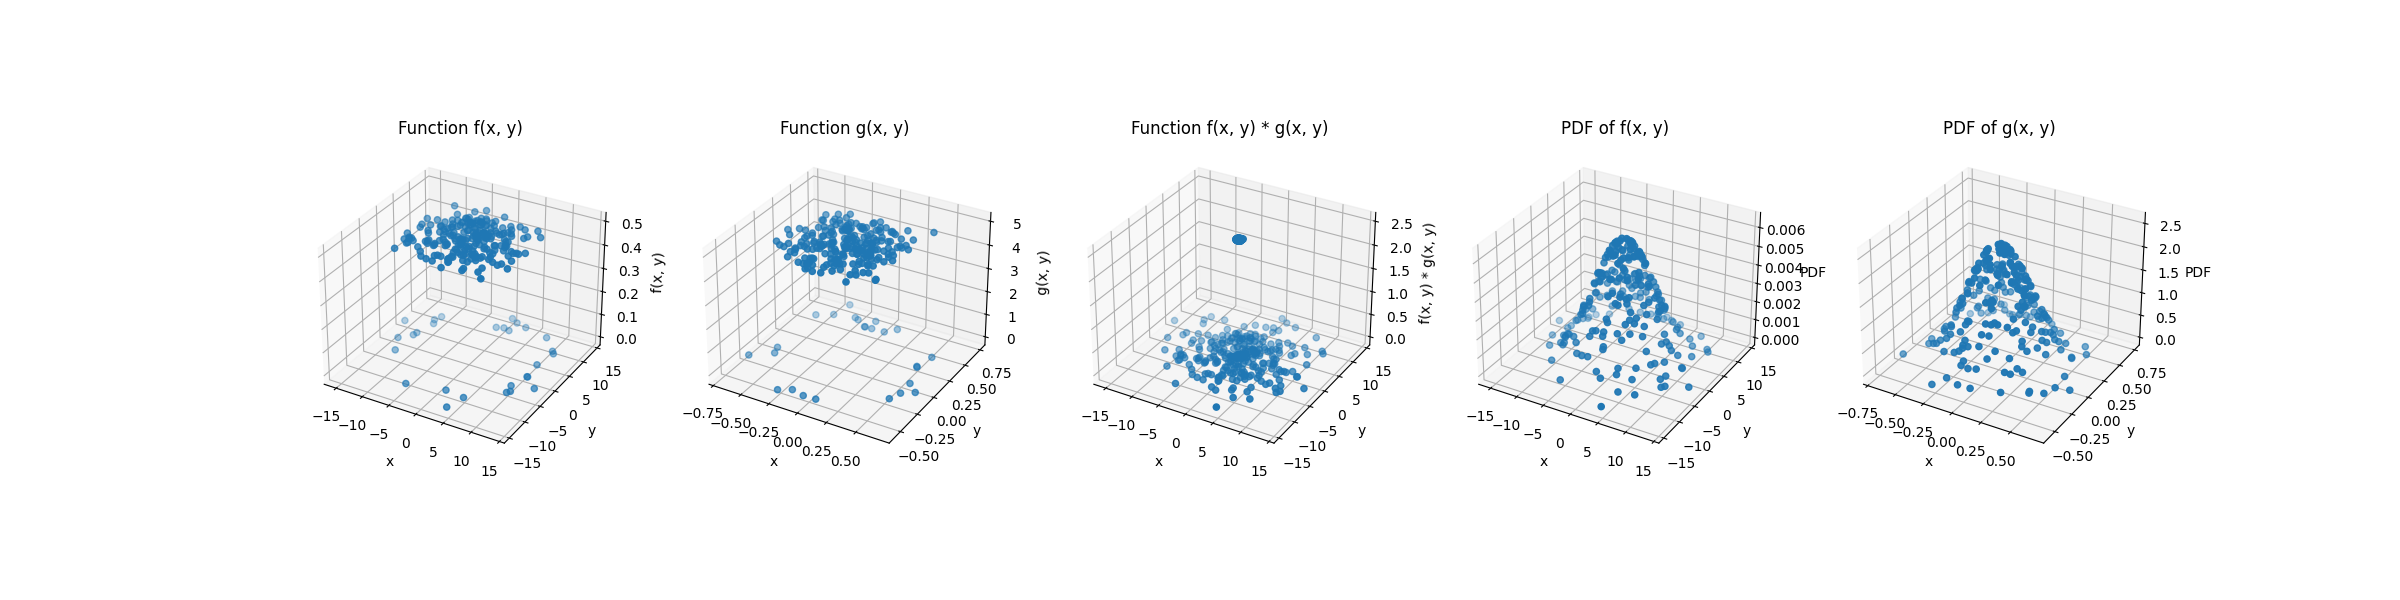
\includegraphics[width=1\textwidth]{balance_heuristic.png}
\caption{Funciones \( f(x) \) y \( g(x) \) en sus respectivos hipercubos, función \( f(x) \cdot g(x) \) y distribuciones de muestreo \( p_{i}(x) \) para cada rango \( [a_{i}, b_{i}] \).}
\label{fig:mis3}
\end{figure}

\subsubsection{Pruebas realizadas}

Sobre este caso de prueba se generó un análisis de las distintas heurísticas implementadas.
El análisis de este ejemplo se hizo de manera diferente a los anteriores y se corrieron todos los tests con los mismos hipercubos.
Entonces:
\begin{itemize}
\item Se hicieron 10 tests diferentes. Para cada test se utilizaron los mismos valores para \( a_{fi} \), \( b_{fi} \), \( c_f \), \( a_{gi} \), \( b_{gi} \) y \( c_g \).
      Los valores para \( a_{fi} \) y \( b_{fi} \) son -10 y 10 respectivamente. \( c_f \) es 0.5.
      Los valores para \( a_{gi} \) y \( b_{gi} \) son -0.5 y 0.5 respectivamente. \( c_g \) es 5.
\item La dimensionalidad de los tests es \( n + 1 \) donde \( n \) toma los siguientes valores: 2, 3, 4, 5, 6, 10, 12, 15, 18, 20.
\item Para cada test se corrió MIS con las siguientes heurísticas: \textit{balance heuristic}, \textit{power heuristic}, \textit{maximum heuristic} y \textit{cutoff heuristic}.
\item Para cada heurística se corrió MIS con 25, 50, 100, 500, 1000, 5000 y 50000 muestras.
\item Para cada heurística y cantidad de muestras se corrió MIS 100 veces y se calculó el promedio de las estimaciones,
      el promedio de la varianza de las estimaciones y el promedio de las desviaciones estándar de las estimaciones.
      A su vez, se calculó el promedio de los errores comparados el valor exacto de la integral y el promedio del tiempo de cómputo.
\end{itemize}

Luego, el análisis se hizo de la misma manera que en las pruebas anteriores.

\subsubsection{Resultados}

\begin{table}[H]
\centering
\label{table:heuristic_sample_analysis}
\small
\setlength{\tabcolsep}{3pt}
\renewcommand{\arraystretch}{1.2}
\begin{tabular}{|l|r|r|r|r|r|r|r|}
\hline
\textbf{\makecell{Heurística / \\ \# de muestras}} & \textbf{25} & \textbf{50} & \textbf{100} & \textbf{500} & \textbf{1000} & \textbf{5000} & \textbf{50000} \\ \hline
\multicolumn{8}{|c|}{\textbf{Promedio de Var}} \\ \hline
\textit{balance heuristic} & 83.88 & 5.48 & 10.06 & 16.93 & 4.61 & 25.98 & 78.95 \\ \hline
\textit{power heuristic} & 8.37 & 14.03 & 19.82 & 1.74 & 12.64 & 25.50 & 78.43 \\ \hline
\textit{maximum heuristic} & 159.54 & 60.44 & 41.34 & 11.77 & 18.73 & 5.72 & 4.50 \\ \hline
\textit{cutoff heuristic} & 42.11 & 43.85 & 8.61 & 16.80 & 4.83 & 25.96 & 3.60 \\ \hline
\multicolumn{8}{|c|}{\textbf{Promedio de Err}} \\ \hline
\textit{balance heuristic} & 0.76 & 1.11 & 0.94 & 0.93 & 0.96 & 0.73 & 0.34 \\ \hline
\textit{power heuristic} & 1.02 & 1.00 & 0.78 & 1.04 & 0.77 & 0.76 & 0.37 \\ \hline
\textit{maximum heuristic} & -0.41 & -0.31 & -0.60 & -0.46 & -0.50 & -0.67 & -0.83 \\ \hline
\textit{cutoff heuristic} & 1.04 & 0.66 & 1.05 & 0.94 & 0.92 & 0.75 & 0.63 \\ \hline
\multicolumn{8}{|c|}{\textbf{Promedio de DE}} \\ \hline
\textit{balance heuristic} & 1.24 & 0.78 & 0.81 & 0.59 & 0.47 & 0.54 & 0.72 \\ \hline
\textit{power heuristic} & 0.97 & 0.88 & 0.99 & 0.50 & 0.66 & 0.51 & 0.71 \\ \hline
\textit{maximum heuristic} & 1.89 & 1.57 & 1.64 & 1.02 & 0.88 & 0.71 & 0.50 \\ \hline
\textit{cutoff heuristic} & 0.97 & 1.19 & 0.72 & 0.59 & 0.51 & 0.52 & 0.42 \\ \hline
\end{tabular}
\caption{Análisis de los resultados por heurística y cantidad de muestras}
\end{table}

\begin{table}[H]
\centering
\label{table:heuristic_test_analysis}
\resizebox{\textwidth}{!}{%
\begin{tabular}{|c|c|c|c|}
\hline
\textbf{Heurística/Test} & \textbf{Promedio de Var} & \textbf{Promedio de Err} & \textbf{Promedio de DE} \\ \hline
\multicolumn{4}{|c|}{\textbf{Test 1 (3 dimensiones)}} \\ \hline
\textit{balance heuristic} & 4.99 & -0.038 & 0.92 \\ \hline
\textit{power heuristic} & 7.62 & -0.215 & 1.11 \\ \hline
\textit{maximum heuristic} & 17.32 & -2.37 & 1.67 \\ \hline
\textit{cutoff heuristic} & 4.45 & 0.016 & 0.86 \\ \hline
\multicolumn{4}{|c|}{\textbf{Test 2 (4 dimensiones)}} \\ \hline
\textit{balance heuristic} & 112.57 & -0.084 & 1.32 \\ \hline
\textit{power heuristic} & 41.46 & -0.107 & 1.35 \\ \hline
\textit{maximum heuristic} & 312.36 & -2.44 & 2.43 \\ \hline
\textit{cutoff heuristic} & 121.58 & -0.488 & 1.73 \\ \hline
\multicolumn{4}{|c|}{\textbf{Test 3 (5 dimensiones)}} \\ \hline
\textit{balance heuristic} & 30.21 & 0.636 & 0.80 \\ \hline
\textit{power heuristic} & 18.34 & 0.700 & 0.74 \\ \hline
\textit{maximum heuristic} & 30.56 & -0.766 & 1.14 \\ \hline
\textit{cutoff heuristic} & 29.77 & 0.609 & 0.80 \\ \hline
\multicolumn{4}{|c|}{\textbf{Test 4 (6 dimensiones)}} \\ \hline
\textit{balance heuristic} & 38.13 & 0.814 & 0.68 \\ \hline
\textit{power heuristic} & 37.52 & 0.820 & 0.68 \\ \hline
\textit{maximum heuristic} & 6.52 & -0.206 & 0.72 \\ \hline
\textit{cutoff heuristic} & 40.02 & 0.735 & 0.76 \\ \hline
\multicolumn{4}{|c|}{\textbf{Test 5 (7 dimensiones)}} \\ \hline
\textit{balance heuristic} & 109.74 & 0.655 & 0.87 \\ \hline
\textit{power heuristic} & 109.28 & 0.686 & 0.85 \\ \hline
\textit{maximum heuristic} & 2.66 & -0.104 & 0.66 \\ \hline
\textit{cutoff heuristic} & 0.38 & 1.217 & 0.32 \\ \hline
\end{tabular}%
}
\caption{Análisis de los resultados por heurística en los tests 1-5}
\end{table}

\begin{table}[H]
\centering
\label{table:heuristic_test_analysis}
\resizebox{\textwidth}{!}{%
\begin{tabular}{|c|c|c|c|}
\hline
\textbf{Heurística/Test} & \textbf{Promedio de Var} & \textbf{Promedio de Err} & \textbf{Promedio de DE} \\ \hline
\multicolumn{4}{|c|}{\textbf{Test 6 (11 dimensiones)}} \\ \hline
\textit{balance heuristic} & 1.68 & 1.265 & 0.41 \\ \hline
\textit{power heuristic} & 2.27 & 1.190 & 0.46 \\ \hline
\textit{maximum heuristic} & 2.10 & 0.095 & 0.77 \\ \hline
\textit{cutoff heuristic} & 1.19 & 1.234 & 0.43 \\ \hline
\multicolumn{4}{|c|}{\textbf{Test 7 (13 dimensiones)}} \\ \hline
\textit{balance heuristic} & 0.88 & 1.294 & 0.44 \\ \hline
\textit{power heuristic} & 2.60 & 1.243 & 0.48 \\ \hline
\textit{maximum heuristic} & 3.59 & 0.072 & 0.86 \\ \hline
\textit{cutoff heuristic} & 1.18 & 1.256 & 0.48 \\ \hline
\multicolumn{4}{|c|}{\textbf{Test 8 (16 dimensiones)}} \\ \hline
\textit{balance heuristic} & 2.77 & 1.259 & 0.54 \\ \hline
\textit{power heuristic} & 2.11 & 1.265 & 0.55 \\ \hline
\textit{maximum heuristic} & 11.72 & -0.016 & 1.13 \\ \hline
\textit{cutoff heuristic} & 5.39 & 1.199 & 0.61 \\ \hline
\multicolumn{4}{|c|}{\textbf{Test 9 (19 dimensiones)}} \\ \hline
\textit{balance heuristic} & 4.73 & 1.264 & 0.63 \\ \hline
\textit{power heuristic} & 2.87 & 1.302 & 0.60 \\ \hline
\textit{maximum heuristic} & 5.19 & 0.405 & 0.88 \\ \hline
\textit{cutoff heuristic} & 0.72 & 1.414 & 0.47 \\ \hline
\multicolumn{4}{|c|}{\textbf{Test 10 (21 dimensiones)}} \\ \hline
\textit{balance heuristic} & 17.01 & 1.180 & 0.75 \\ \hline
\textit{power heuristic} & 5.24 & 1.314 & 0.64 \\ \hline
\textit{maximum heuristic} & 39.47 & -0.077 & 1.45 \\ \hline
\textit{cutoff heuristic} & 3.54 & 1.375 & 0.56 \\ \hline
\end{tabular}%
}
\caption{Análisis de los resultados por heurística en los tests 6-10}
\end{table}

\begin{table}[H]
\centering
\label{table:heuristic_analysis}
\begin{tabular}{|c|c|c|c|}
\hline
\textbf{Heurística} & \textbf{Promedio de Var} & \textbf{Promedio de Err} & \textbf{Promedio de DE} \\ \hline
\textit{balance heuristic} & 32.27 & 0.825 & 0.736 \\ \hline
\textit{power heuristic} & 22.93 & 0.820 & 0.746 \\ \hline
\textit{maximum heuristic} & 43.15 & -0.541 & 1.172 \\ \hline
\textit{cutoff heuristic} & 20.82 & 0.857 & 0.704 \\ \hline
\end{tabular}
\caption{Análisis de los resultados por heurística}
\end{table}


\subsubsection{Análisis}

\paragraph{Varianza de las Estimaciones}
En términos de varianza, la heurística \textit{balance heuristic} muestra un rendimiento consistentemente bueno, con una disminución notable en la varianza al aumentar el tamaño de la muestra. Por el contrario, \textit{maximum heuristic} muestra la mayor variabilidad, lo que sugiere una menor fiabilidad y estabilidad en sus resultados.

\paragraph{Error de las Estimaciones}
Respecto a los errores, \textit{balance heuristic} mantiene errores bajos y consistentes a través de los diferentes tamaños de muestra, lo que implica una mayor precisión en sus estimaciones. En cambio, \textit{maximum heuristic} se inclina hacia errores negativos, indicando una tendencia a la subestimación. \textit{cutoff heuristic} y \textit{power heuristic} muestran más variabilidad en sus errores, lo que sugiere una precisión menos consistente.

\paragraph{Desviaciones Estándar de las Estimaciones}
Las desviaciones estándar más bajas se observan en la heurística \textit{balance heuristic}, lo que señala una mayor precisión y fiabilidad en sus estimaciones. \textit{power heuristic}, \textit{maximum heuristic}, y \textit{cutoff heuristic} muestran desviaciones estándar más altas y variables, lo que refleja una consistencia y precisión menos fiables.

\paragraph{Dimensionalidad}
La dimensionalidad afecta significativamente el rendimiento de las heurísticas. En dimensiones más bajas, todas las heurísticas muestran un buen rendimiento. Sin embargo, en dimensiones más altas, \textit{balance heuristic} logra mantener un control más efectivo sobre la varianza y el error, mientras que \textit{maximum heuristic} y \textit{cutoff heuristic} experimentan un aumento significativo en la varianza y el error.

\paragraph{Conclusiones}
En resumen, \textit{balance heuristic} emerge como la heurística más robusta y consistente en la Prueba 3, demostrando una buena precisión y estabilidad a lo largo de diferentes tamaños de muestra y en varias dimensiones. En contraste, \textit{maximum heuristic} muestra una tendencia a la subestimación y es menos confiable, especialmente en dimensiones más altas. \textit{power heuristic} y \textit{cutoff heuristic} ofrecen un rendimiento intermedio, pero su precisión y consistencia son menos predecibles en comparación con \textit{balance heuristic}.

\section{Conclusiones}

Las pruebas realizadas en este trabajo muestran que el MIS es una buena técnica para la estimación de distintas integrales.
Se probó en un espacio amplio de dimensiones y con distintas heurísticas en cada caso.

El caso 1, que es el más simple, mostró que el MIS es efectivo en dimensiones bajas y que la heurística \textit{balance heuristic} es la más efectiva.
Este caso fue útil para entender cómo funciona el MIS y cómo se comporta en un caso simple.

El caso 2, que es un caso más complejo, dio la posibilidad de probar una heurística nueva (\textit{sbert heuristic}) y ver como su varianza y desviación estándar son levemente menores a las otras heurísticas.

El caso 3, nos ayudó a entender cómo funciona el MIS en un producto de hipercubos y cómo se comporta en dimensiones más altas.
Sirvió para hacer un análisis en donde se multiplica una función de baja integral con una de alta integral y ver cómo el MIS se comporta en este caso.
De vuelta, la heurística \textit{balance heuristic} mostró ser la más efectiva.

En resumen, el MIS es una técnica efectiva para la estimación de integrales en espacios de alta dimensión y la heurística \textit{balance heuristic} es la más efectiva en la mayoría de los casos.
Se vio que la heurística presentada por Sbert también es efectiva en la mayoría de los casos y que se comporta de manera muy similar a \textit{balance heuristic}.

Se pudo observar que las funciones utilizadas claramente no aportan el contexto necesario para que las heurísticas \textit{power heuristic} \textit{maximum heuristic} y \textit{cutoff heuristic}.
Como explicado en las primeras secciones, estas heurísticas son efectivas en contextos muy particulares que no son reflejados en estos casos de prueba.

Para más información se puede ver el repositorio de GitHub en el que se encuentra el código utilizado para este trabajo: \url{https://github.com/santiagolmedo/multiple_importance_sampling}.
En él, se encuentran los códigos utilizados para las pruebas y los todos los resultados obtenidos.

\begin{thebibliography}{99}

\bibitem{Veach1997}
Eric Veach (1997) \emph{Multiple Importance Sampling}, Chapter 9 in Ph.D. thesis, Stanford University. [Online]. Available: \url{https://graphics.stanford.edu/courses/cs348b-03/papers/veach-chapter9.pdf}

\bibitem{Sbert2016}
M. Sbert, V. Havran, László Szirmay-Kalos (2016) \emph{Variance Analysis of Multi-sample and One-sample Multiple Importance Sampling}, Computer Graphics Forum, Vol. 35, No. 7, DOI: 10.1111/cgf.13042. [Online]. Available: \url{https://dx.doi.org/10.1111/cgf.13042}

\bibitem{Kajiya1986}
James T. Kajiya (1986) \emph{The Rendering Equation}, ACM SIGGRAPH Computer Graphics, Vol. 20, No. 4, pp. 143-150. [Online]. Available: \url{https://dl.acm.org/doi/pdf/10.1145/15922.15902}

\end{thebibliography}

\end{document}

\[ (\int_{\Omega} \sum_{i=1}^{n} \frac{w_{i}^{2}(x) * f^{2}(x)}{n_{i} * p_{i}(x)} \,d\mu(x)) - (\sum_{i=1}^{n} \frac{1}{n_{i}} * \mu_{i}^{2}) \]

where

\[ \mu_{i} = \int_{\Omega} w_{i}(x) * f(x) \,d\mu(x)\]

$1 \times 10^{6}$